\documentclass{article}

% these packages let you do math
\usepackage{amsmath}
\usepackage{amssymb}

% we need these packages for fancy R tables
\usepackage{booktabs}
\usepackage{float}
\usepackage{colortbl}
\usepackage{xcolor}

% these packages play with the spacing/margins of the document. Uncomment the commands on lines 16 and 17 to see what they do.
\usepackage{a4wide}
\usepackage{setspace}
\usepackage{geometry}
\usepackage{parskip}
%\doublespacing
%\geometry{margin=1.5in}

% this package helps us with including images. Setting the graphics path makes it easier to refer to things in the \includegraphics command.
\usepackage{graphicx}
\graphicspath{ {../figures/} }

% make some hyperlinks using the \href command
\usepackage{hyperref}
\hypersetup{
    colorlinks=true,
    linkcolor=black,
    urlcolor=blue
}

% set the author, title, and date of the document. \maketitle adds it to the document.
\author{Afif Mazhar}
\title{My Paper on NLSY02 Data}
\date{Sping 2022}

\begin{document}
\maketitle

\section{Data}

We will be analyzing the dataset of National Longitudinal Survey of Youth from 1997. The data set reflects incarceration rates from the year 2002 and the respective gender/race associated with incarceration.
\newpage

\section{Analysis}

In order to provide qualitative analysis over the dataset given, included is three visualizations that depict the data uniquely. Figure 1 portrays the mean number of incarcerations per respective demographic in the year 2002. Figure 2 quantifies the previous visualization, and Figure 3 is a regressed form of the entire dataset.


\begin{figure}[H]
    \begin{center}
        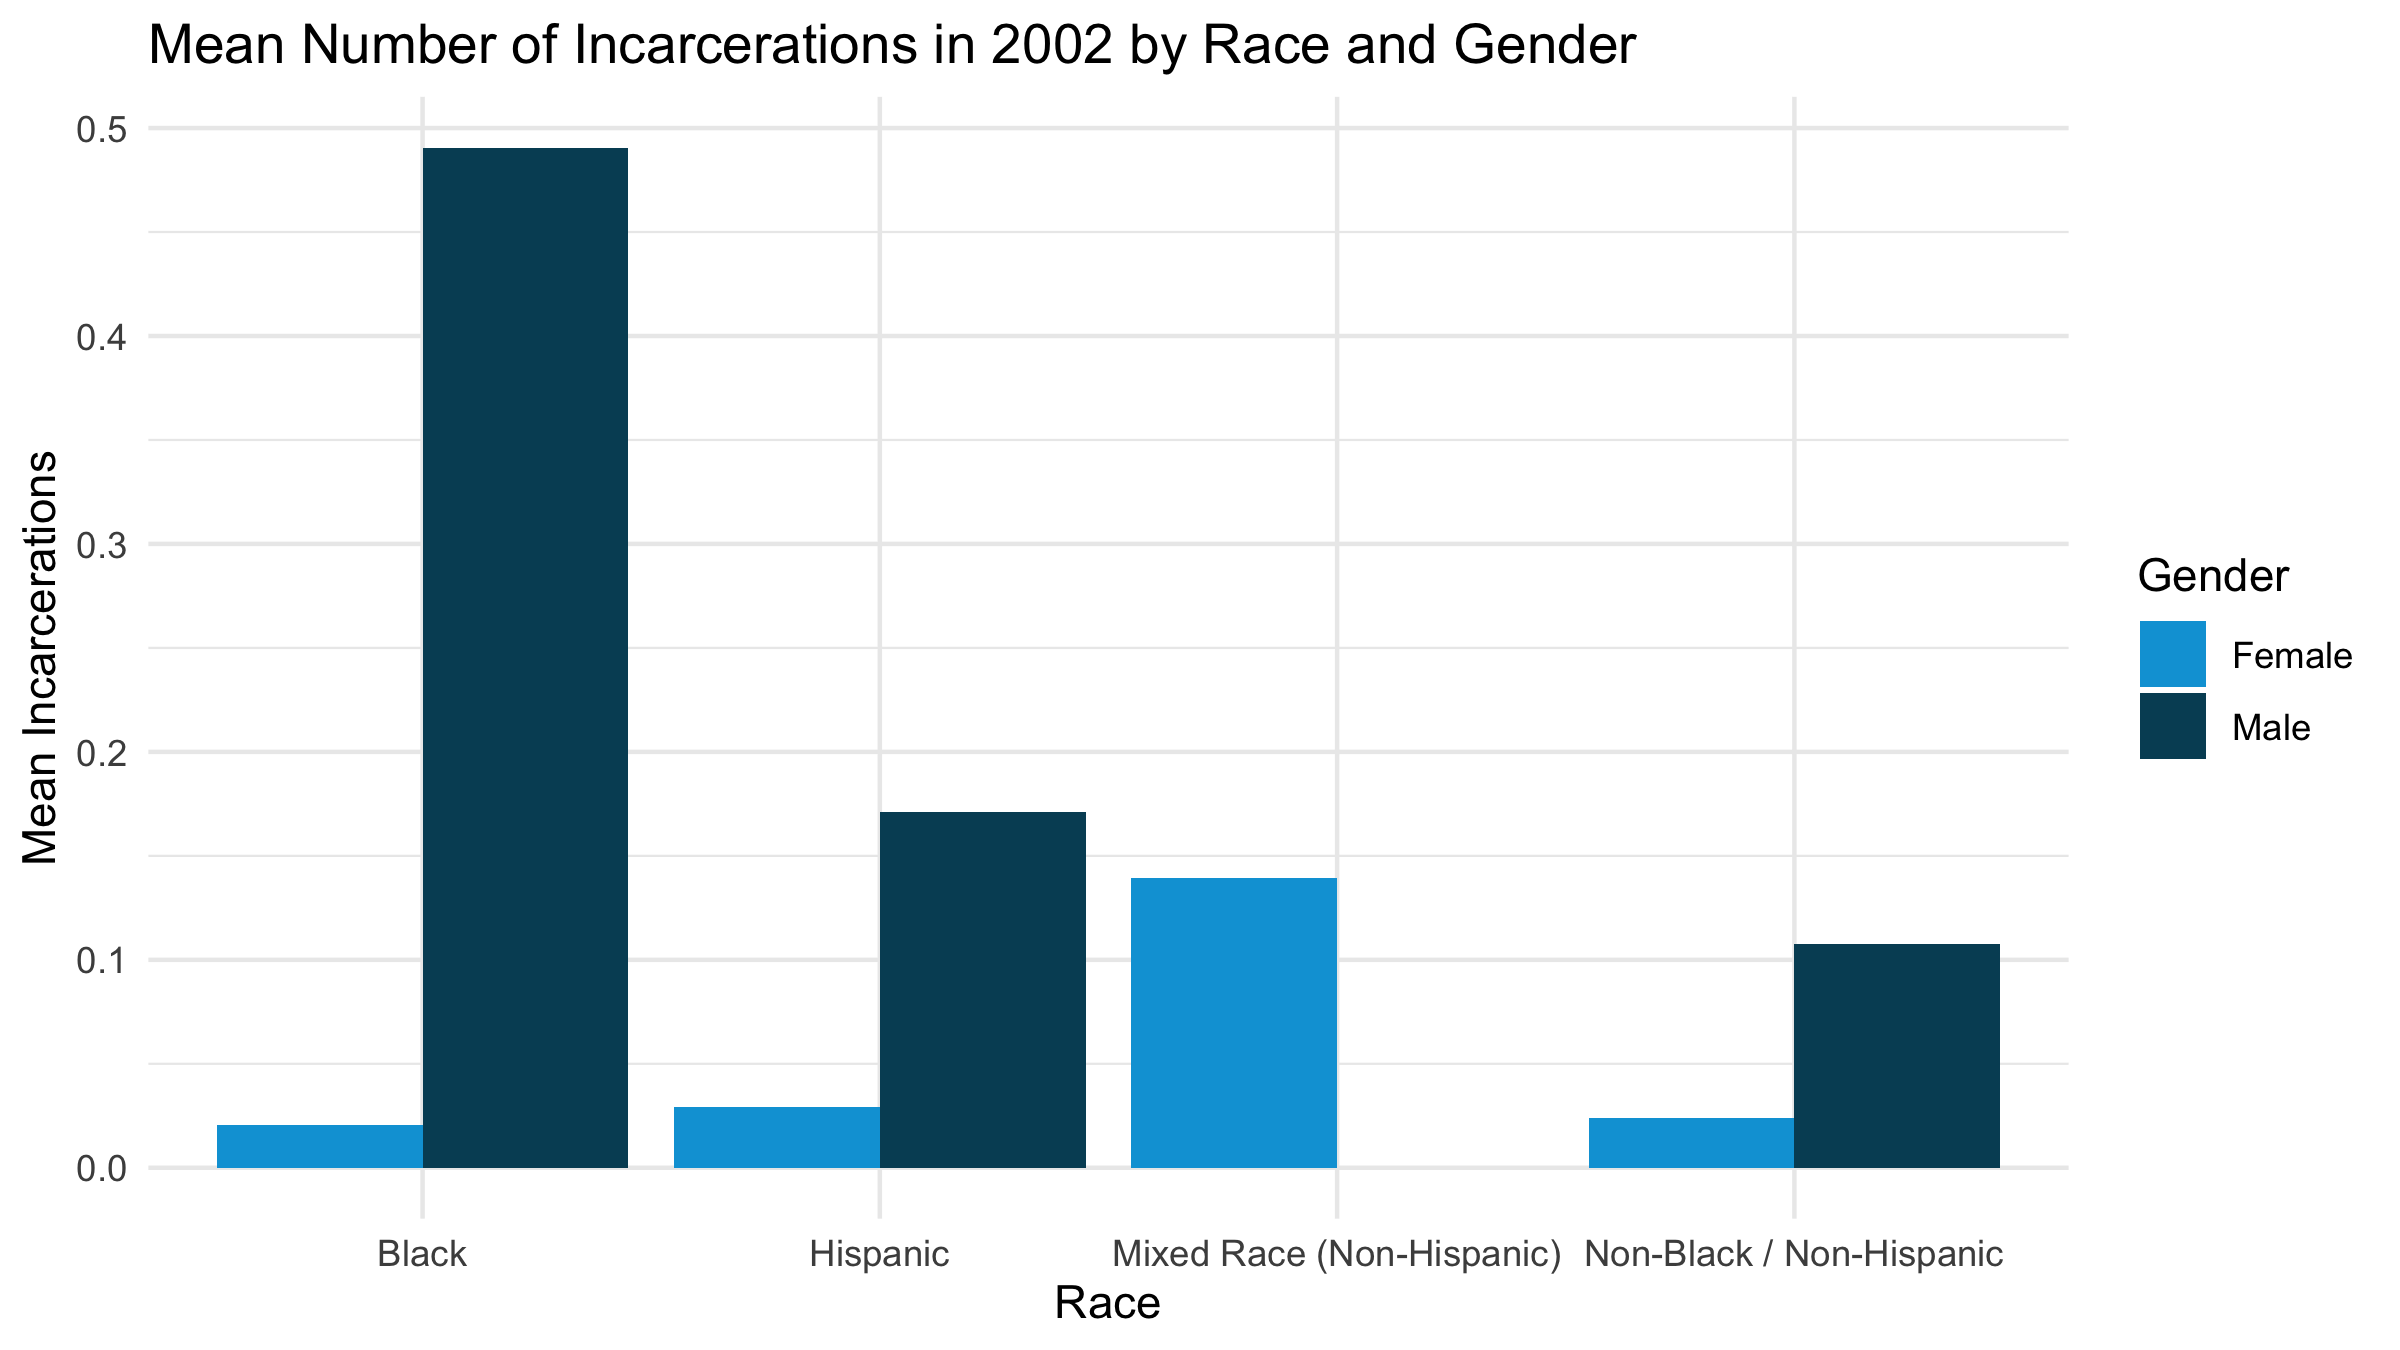
\includegraphics[width=.85\textwidth]{incarcerations_by_racegender}
    \end{center}
    \caption{Mean Number of Incarcerations in 2002 by Race and Gender}
    \label{fig:graph}
\end{figure}


As displayed above, the largest mean of incarcerations is Black Male with an average of 0.49 (reflected numerically below in Table 1). Non-black/Non-Hispanic females are the higher mean comparative to the men in the respective category with a 0.107 average. Mixed Race (Non-Hispanic) males are non-existent in Figure 1. Table 2 depicts a regression output of the dataset where Hispanic, Mixed Race, and the Non-Black categories are have a negative coefficient. This indicates that there is a negative relationship with the increase in the number of incarcerations and the respective category depicted over 8,978 observations. The Male category, however, shows a positive relationship with incarcerations. This indicates as the amount of incarcerations increase by 0.01, there is a 0.194 increase in the amount of males incarcerated. The r-squared value is very low so this regression does not provide perfect, accurate measures of the regression at hand.

\begin{table}[H]

\caption{\label{tab:tab:summarystats}Mean incarcerations in 2002 by Race and Gender}
\centering
\begin{tabular}[t]{lrrrr}
\toprule
Gender & Black & Hispanic & Mixed Race Non Hispanic & Non Black Non Hispanic\\
\midrule
\cellcolor{gray!6}{Female} & \cellcolor{gray!6}{0.0206009} & \cellcolor{gray!6}{0.0292524} & \cellcolor{gray!6}{0.1395349} & \cellcolor{gray!6}{0.0240000}\\
Male & 0.4905822 & 0.1709314 & 0.0000000 & 0.1073798\\
\bottomrule
\end{tabular}
\end{table}



% Table created by stargazer v.5.2.2 by Marek Hlavac, Harvard University. E-mail: hlavac at fas.harvard.edu
% Date and time: Fri, Feb 18, 2022 - 01:57:51
\begin{table}[!htbp] \centering 
  \caption{Regression Output. Omitted category is Black Females.} 
  \label{tab:regression} 
\begin{tabular}{@{\extracolsep{5pt}}lc} 
\\[-1.8ex]\hline 
\hline \\[-1.8ex] 
 & \multicolumn{1}{c}{\textit{Dependent variable:}} \\ 
\cline{2-2} 
\\[-1.8ex] & Incarcerations in 2002 \\ 
\hline \\[-1.8ex] 
 Hispanic & $-$0.156$^{***}$ \\ 
  & (0.039) \\ 
  & \\ 
 Mixed Race (Non-Hispanic) & $-$0.180$^{**}$ \\ 
  & (0.081) \\ 
  & \\ 
 Non-Black / Non-Hispanic & $-$0.192$^{***}$ \\ 
  & (0.034) \\ 
  & \\ 
 Male & 0.194$^{***}$ \\ 
  & (0.022) \\ 
  & \\ 
 Constant & 0.159$^{***}$ \\ 
  & (0.025) \\ 
  & \\ 
\hline \\[-1.8ex] 
Observations & 8,978 \\ 
R$^{2}$ & 0.014 \\ 
Adjusted R$^{2}$ & 0.014 \\ 
Residual Std. Error & 1.050 (df = 8973) \\ 
F Statistic & 32.087$^{***}$ (df = 4; 8973) \\ 
\hline 
\hline \\[-1.8ex] 
\textit{Note:}  & \multicolumn{1}{r}{$^{*}$p$<$0.1; $^{**}$p$<$0.05; $^{***}$p$<$0.01} \\ 
\end{tabular} 
\end{table} 


\end{document}
